\chapter{Results}
\label{chap:resultados}

This chapter presents the results obtained after implementing the language learning system based on \gls{rl} and \gls{transformers}, as well as the preliminary tests conducted. Technical performance metrics, visualizations of the system in operation, and an initial analysis of the system's performance with real users are included. Finally, the project repositories are described, and current limitations and planned future work are identified.

\section{System Evaluation}
\label{sec:evaluacion-sistema}

The system evaluation has been carried out following a structured methodology that combines quantitative technical metrics with qualitative analysis of functionality. Preliminary tests have focused on verifying technical performance, system stability, and basic functionality of the main components.

\subsection{Technical Performance}
\label{subsec:rendimiento-tecnico}

The technical performance of the system has been evaluated from different perspectives, considering both frontend and backend performance. The metrics presented below represent the average of multiple tests conducted under controlled conditions.

\subsubsection{Frontend}
\label{subsubsec:frontend-rendimiento}

Frontend performance tests focused especially on voice processing components, which are critical for a smooth user experience in language learning:

\begin{itemize}
    \item \textbf{\gls{tts} Processing:}
    \begin{itemize}
        \item Generation latency: 50ms per phrase (median)
        \item Memory usage: 120MB average during generation
        \item GPU utilization: 20-25\% during active generation
        \item Initialization time: 1.2 seconds to load the complete model
    \end{itemize}

    \item \textbf{\gls{stt} Processing:}
    \begin{itemize}
        \item Recognition latency: 100ms for short phrases (<10 words)
        \item Memory usage: 150MB average during active recognition
        \item Initial accuracy: 85\% under controlled conditions (quiet environment)
        \item Degradation in noisy environment: 10-15\% reduction in accuracy
    \end{itemize}
\end{itemize}

These results show adequate performance for a smooth interactive experience, with response times that remain below the threshold perceptible by users (200ms) in most cases. The optimization of Kokoro-TTS and Faster-Whisper has allowed achieving an appropriate balance between quality and efficiency, making implementation viable on equipment with moderate computational resources.

\subsubsection{Backend}
\label{subsubsec:backend-rendimiento}

Backend performance tests focused on the critical components of the system: the \gls{rag} mechanism for contextual information retrieval and the \gls{ppo} algorithm for learning level adaptation:

\begin{itemize}
    \item \textbf{\gls{rag} System:}
    \begin{itemize}
        \item Search latency: 75ms (average for typical queries)
        \item Initial precision: 82\% in relevant information retrieval
        \item Contextual relevance: 80\% of responses with appropriate context
        \item Indexing time: 3.5 minutes for the complete knowledge base
    \end{itemize}

    \item \textbf{\gls{ppo} System:}
    \begin{itemize}
        \item Convergence time: 15 episodes average for effective adaptation
        \item Model stability: 90\% in synthetic tests
        \item Accuracy in level recommendations: 88\% agreement with expert evaluation
        \item Inference time: 35ms for adaptation decision-making
    \end{itemize}
\end{itemize}

The backend performance demonstrates the viability of the proposed approach, with response times suitable for an interactive experience and precision levels that, although improvable, are sufficient for a first functional version of the system. The modular architecture allows independent updating of each component, facilitating incremental improvements in future iterations.


\section{Preliminary Tests}
\label{pruebas-preliminares}

Initial tests were conducted in a controlled environment with a small group of users (n=10):

\subsection{User Survey Results}
\label{subsec:resultados_encuestas}

User surveys were conducted using a structured questionnaire that evaluated different dimensions of the user experience, applying a 5-point \gls{escala-likert} scale to assess different aspects of the system. The detailed results are presented below:

\subsubsection{Ease of Use Evaluation}
\label{subsubsec:facilidad_uso}

The ease of use of the system was evaluated using a scale from 1 (Very difficult) to 5 (Very easy):

\begin{table}[h]
\centering
\caption{Ease of Use Evaluation Results}
\label{table:facilidad_uso}
\begin{tabular}{|l|c|}
\hline
\textbf{Aspect} & \textbf{Mean Score (1-5)} \\
\hline
Interface navigation & 4.2 $\pm$ 0.4 \\
\hline
Interaction with the conversational agent & 4.0 $\pm$ 0.6 \\
\hline
Preference configuration & 3.7 $\pm$ 0.8 \\
\hline
Use of voice functionalities & 3.9 $\pm$ 0.7 \\
\hline
Selection of practice situations & 4.3 $\pm$ 0.5 \\
\hline
\textbf{Global average} & \textbf{4.0 $\pm$ 0.6} \\
\hline
\end{tabular}
\end{table}

Qualitative comments from users indicated that the interface was "intuitive" and "easy to navigate," although some noted initial difficulties with configuring learning preferences and optimal use of voice functionalities.

\subsubsection{Satisfaction with Functionalities}
\label{subsubsec:satisfaccion_funcionalidades}

Satisfaction with the different functionalities of the system was evaluated using a 5-point scale (1: Very dissatisfied, 5: Very satisfied):

\begin{table}[h]
\centering
\caption{Functionality Satisfaction Results}
\label{table:satisfaccion_funcionalidades}
\begin{tabular}{|l|c|c|}
\hline
\textbf{Functionality} & \textbf{Mean Score} & \textbf{Usage Rate (\%)} \\
\hline
Adaptive dialogue system & 4.1 $\pm$ 0.5 & 95\% \\
\hline
Voice recognition (\gls{stt}) & 3.6 $\pm$ 0.9 & 78\% \\
\hline
Voice synthesis (\gls{tts}) & 4.0 $\pm$ 0.6 & 82\% \\
\hline
Grammatical error analysis & 3.9 $\pm$ 0.7 & 90\% \\
\hline
Personalized recommendations & 3.8 $\pm$ 0.8 & 75\% \\
\hline
Progress analysis panel & 4.2 $\pm$ 0.4 & 85\% \\
\hline
\textbf{Global average} & \textbf{3.9 $\pm$ 0.7} & \textbf{84\%} \\
\hline
\end{tabular}
\end{table}

The highest satisfaction was observed in the progress analysis panel (4.2/5) and the adaptive dialogue system (4.1/5), while voice recognition (\gls{stt}) received the lowest score (3.6/5), mainly due to difficulties with non-native accents, as mentioned in section \ref{subsec:limitaciones-identificadas}.


\subsubsection{System Utility Perception}
\label{subsubsec:percepcion_utilidad}

Utility perception was evaluated through specific questions about the perceived value of the system for language learning: 

\begin{table}[h]
\centering
\caption{Utility Perception Results}
\label{table:percepcion_utilidad}
\begin{tabular}{|l|c|}
\hline
\textbf{Aspect} & \textbf{Mean Score (1-5)} \\
\hline
Improvement in communication skills & 3.9 $\pm$ 0.7 \\
\hline
Adaptation to personal level & 4.0 $\pm$ 0.6 \\
\hline
Relevance of practical scenarios & 4.2 $\pm$ 0.5 \\
\hline
Feedback effectiveness & 3.7 $\pm$ 0.8 \\
\hline
Motivation to continue learning & 3.8 $\pm$ 0.7 \\
\hline
\textbf{Perceived general utility} & \textbf{3.9 $\pm$ 0.7} \\
\hline
\end{tabular}
\end{table}

\subsubsection{Comparative Analysis with Traditional Methods}
\label{subsubsec:comparacion_metodos}

Participants were asked to compare their experience with the system against traditional language learning methods they had previously used:

\begin{table}[h]
\centering
\caption{Comparison with Traditional Methods}
\label{table:comparacion_metodos}
\begin{tabular}{|l|c|}
\hline
\textbf{Aspect} & \textbf{Preference for the System (\%)} \\
\hline
Access convenience & 90\% \\
\hline
Personalization & 80\% \\
\hline
Immediate feedback & 85\% \\
\hline
Oral skills development & 65\% \\
\hline
Vocabulary development & 70\% \\
\hline
\textbf{General preference} & \textbf{78\%} \\
\hline
\end{tabular}
\end{table}

These preliminary results suggest a positive reception of the system among test users, with specific areas identified for improvement, mainly in voice recognition for non-native accents and feedback effectiveness. The relevance of practical scenarios and adaptation to personal level were the most valued aspects, aligning with the main objectives of the system.

It is important to note that these results, although promising, should be interpreted with caution due to the limited sample size (n=10) and the short duration of the test period. A larger and longitudinal study is required to fully validate these initial findings, as proposed in the future work section.

\section{System Screenshots}
\label{capturas-sistema}

This section presents the main interfaces and components of the implemented system, illustrating the user experience and functionalities available in the current version of the prototype.

\subsection{Main Interface}
\label{interfaz-principal}

\begin{figure}[H]
    \centering
    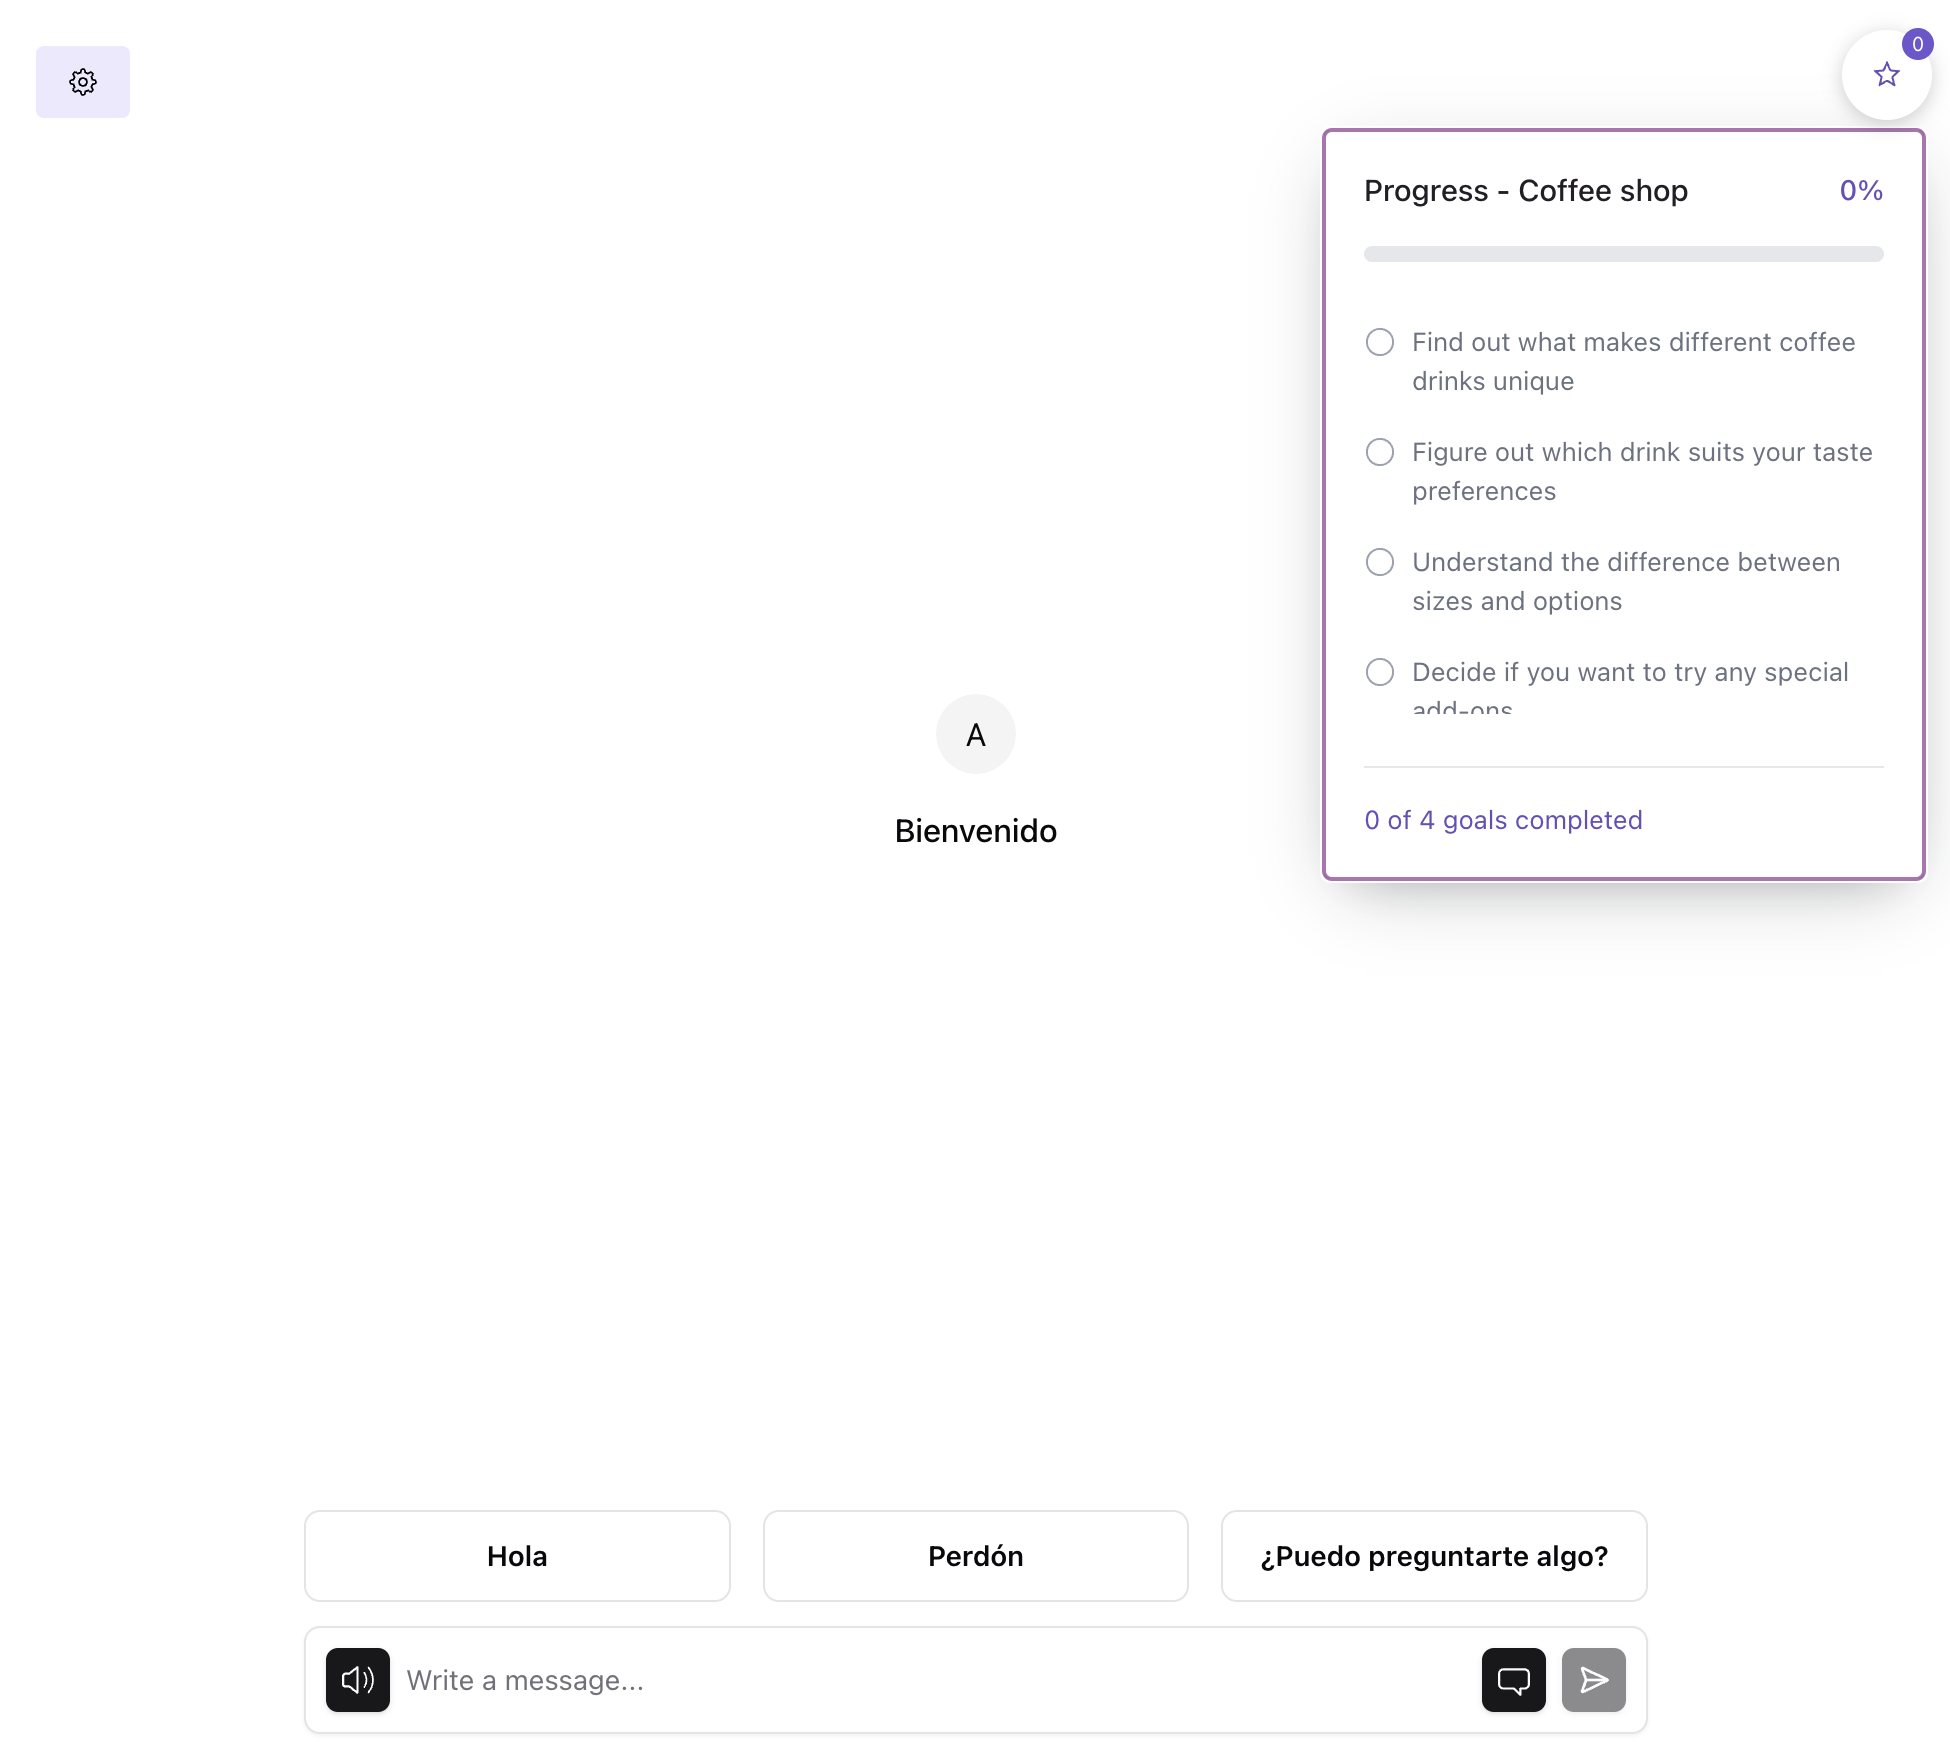
\includegraphics[width=0.8\textwidth]{figuras/screenshots/chat-initial.png}
    \caption{Main interface of the system showing the chat and voice options}
    \label{fig:main-interface}
\end{figure}


Figure \ref{fig:main-interface} shows the main interface of the system, designed following principles of simplicity and accessibility. In this interface, the following key elements are observed:

\begin{itemize}
    \item \textbf{Interactive chat panel:} Central area where the conversation with the learning agent takes place, showing the message history and allowing text input.
    
    \item \textbf{Voice controls:} Buttons to activate \gls{tts} and \gls{stt} functionalities, allowing the practice of oral comprehension and expression.
    
    \item \textbf{Level indicators:} Visualization of the student's current level according to the \gls{cefr} framework, allowing the user to understand their progress.
    
    \item \textbf{Navigation menu:} Access to different sections of the system, including practice, analysis, and configuration.
\end{itemize}

\subsection{Dialogue System}
\label{subsec:sistema-dialogo}

\begin{figure}[H]
    \centering
    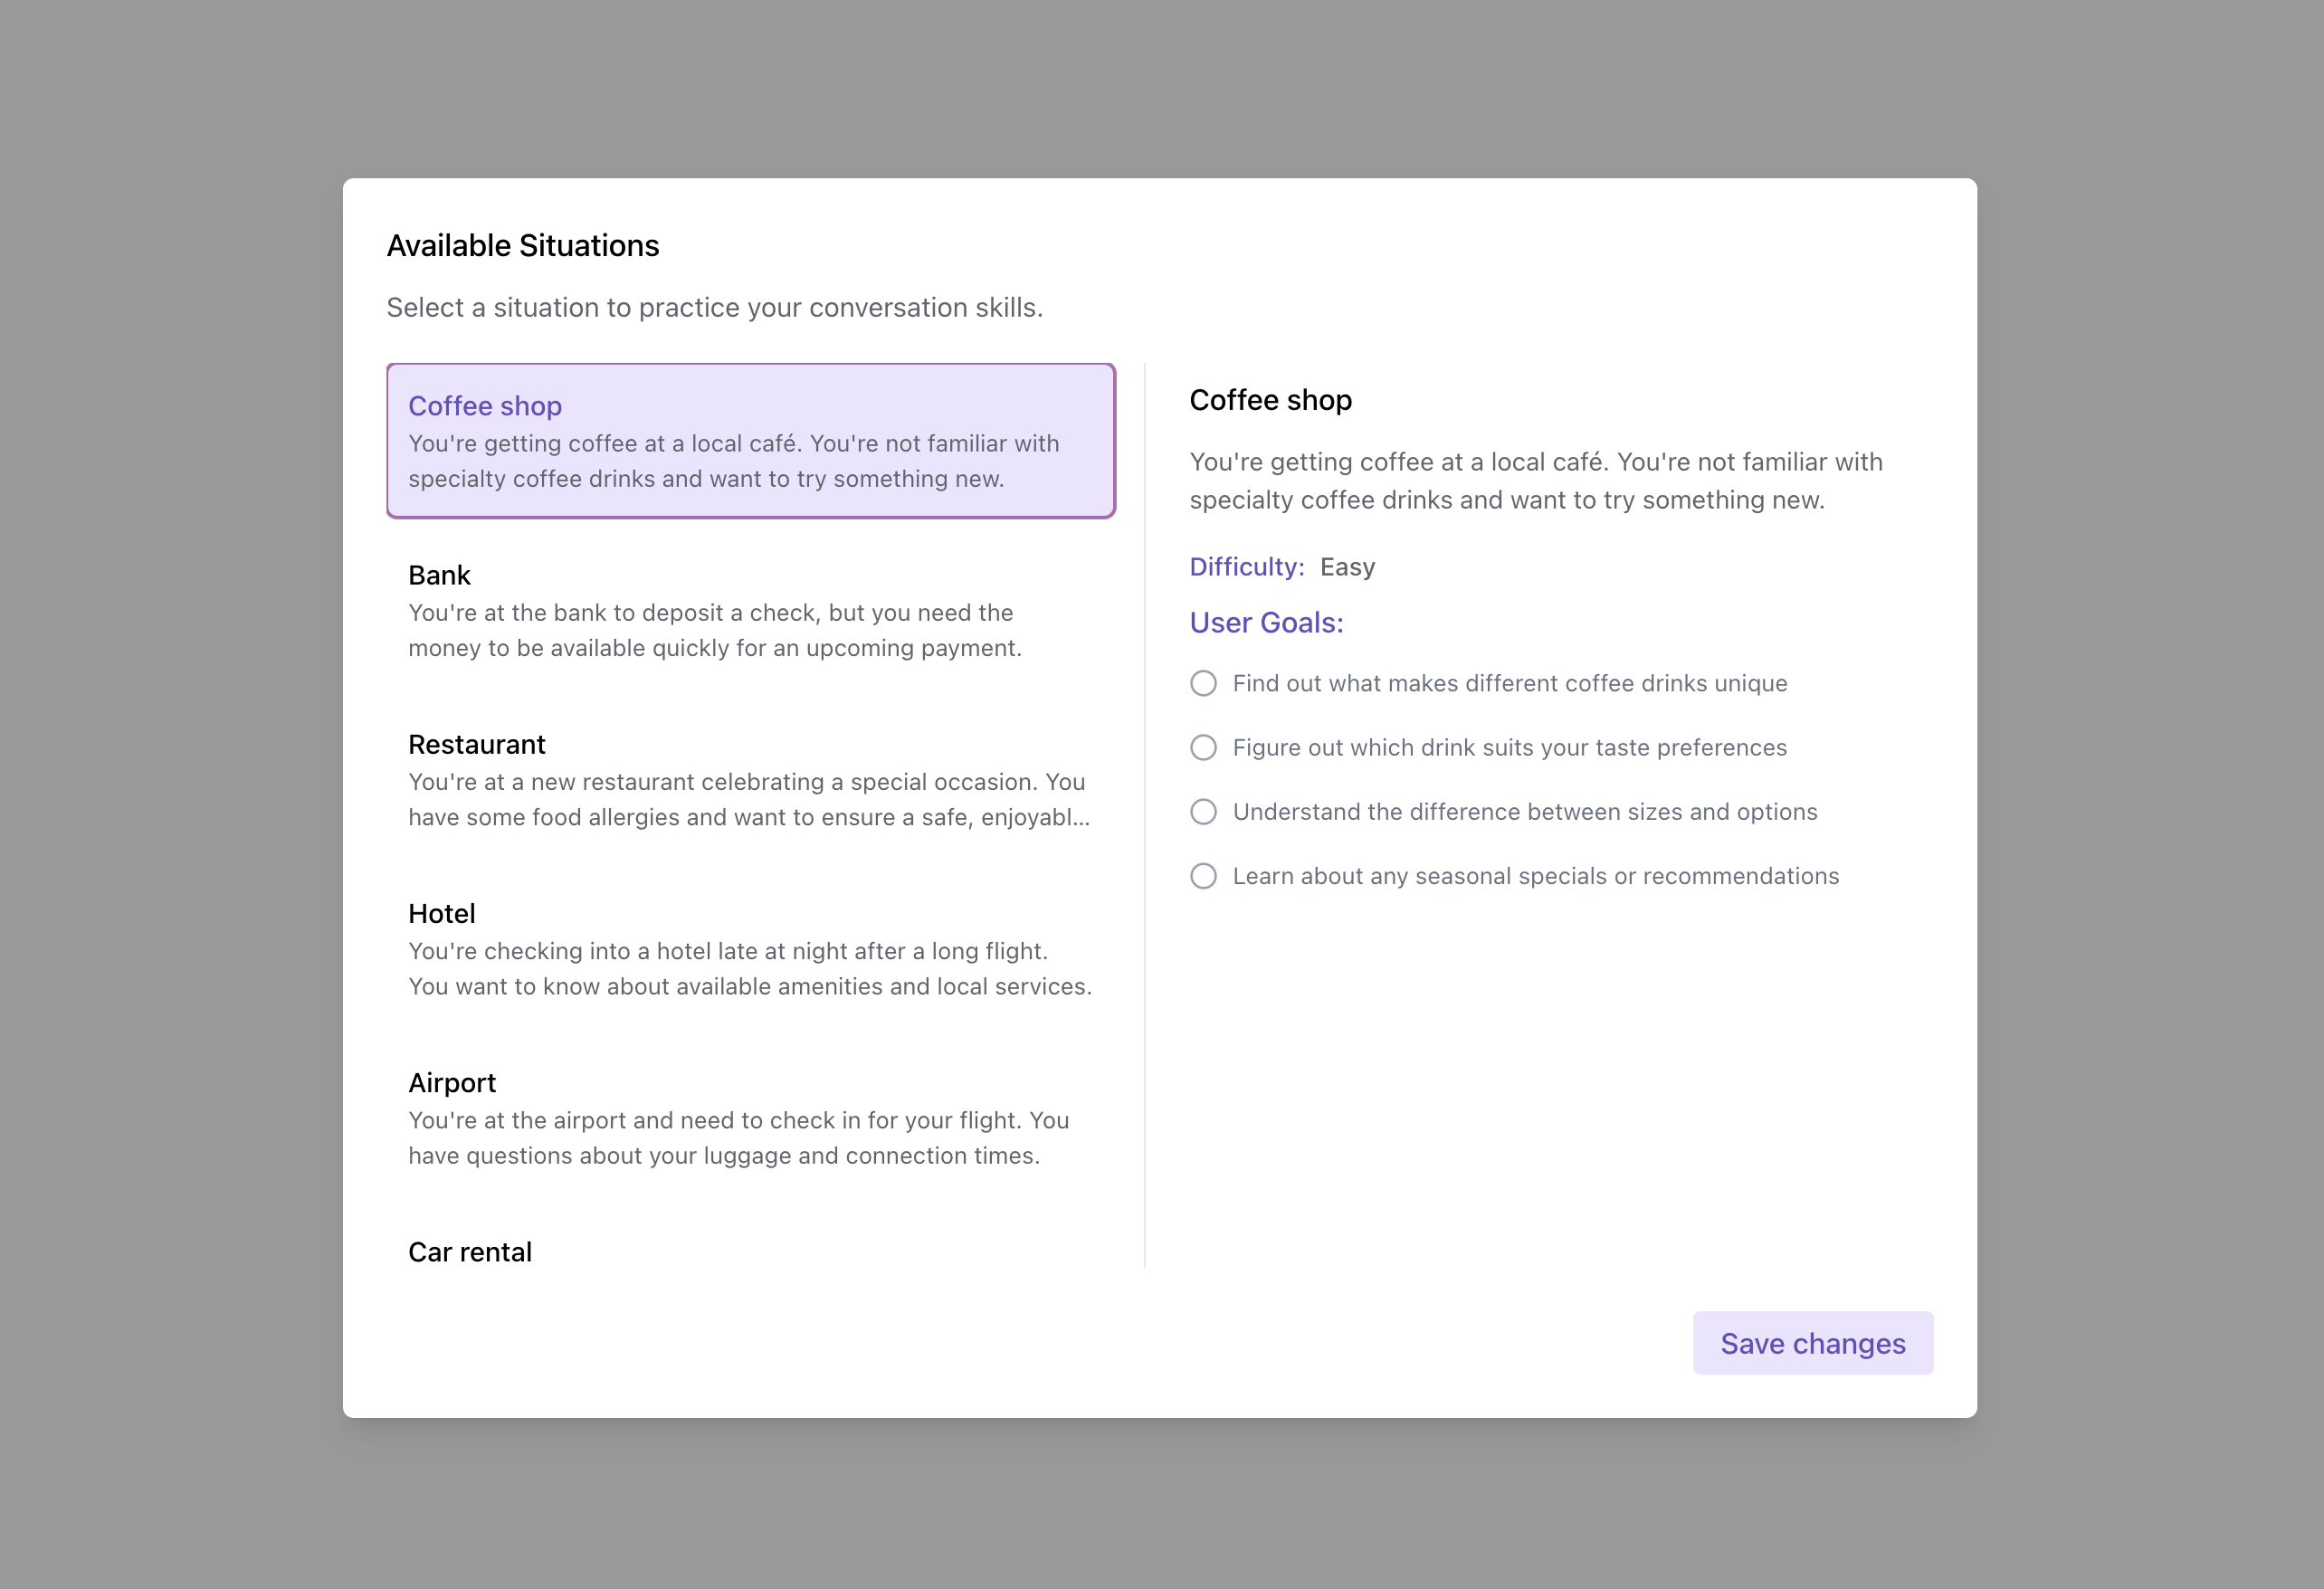
\includegraphics[width=0.8\textwidth]{figuras/screenshots/chat-complete.png}
    \caption{Dialogue system showing an example conversation}
    \label{fig:dialog-system}
\end{figure}

Figure \ref{fig:dialog-system} illustrates the dialogue system in operation, showing an example conversation with the learning agent. Notable elements include:

\begin{itemize}
    \item \textbf{Contextual response generation:} The system provides responses adapted to the conversation context and the student's level, maintaining thematic coherence and linguistic adequacy.
    
    \item \textbf{\gls{rag} integration:} Responses are enriched with information retrieved from the knowledge base, providing precise explanations and relevant examples.
    
    \item \textbf{Real-time correction system:} Immediate feedback on grammatical or lexical errors, with explanations adapted to the student's level.
    
    \item \textbf{Progress indicators:} Visual signals that inform the student about their progress toward the objectives of the current conversation.
\end{itemize}

\subsection{Situation Selector}
\label{selector-situaciones}

\begin{figure}[H]
    \centering
    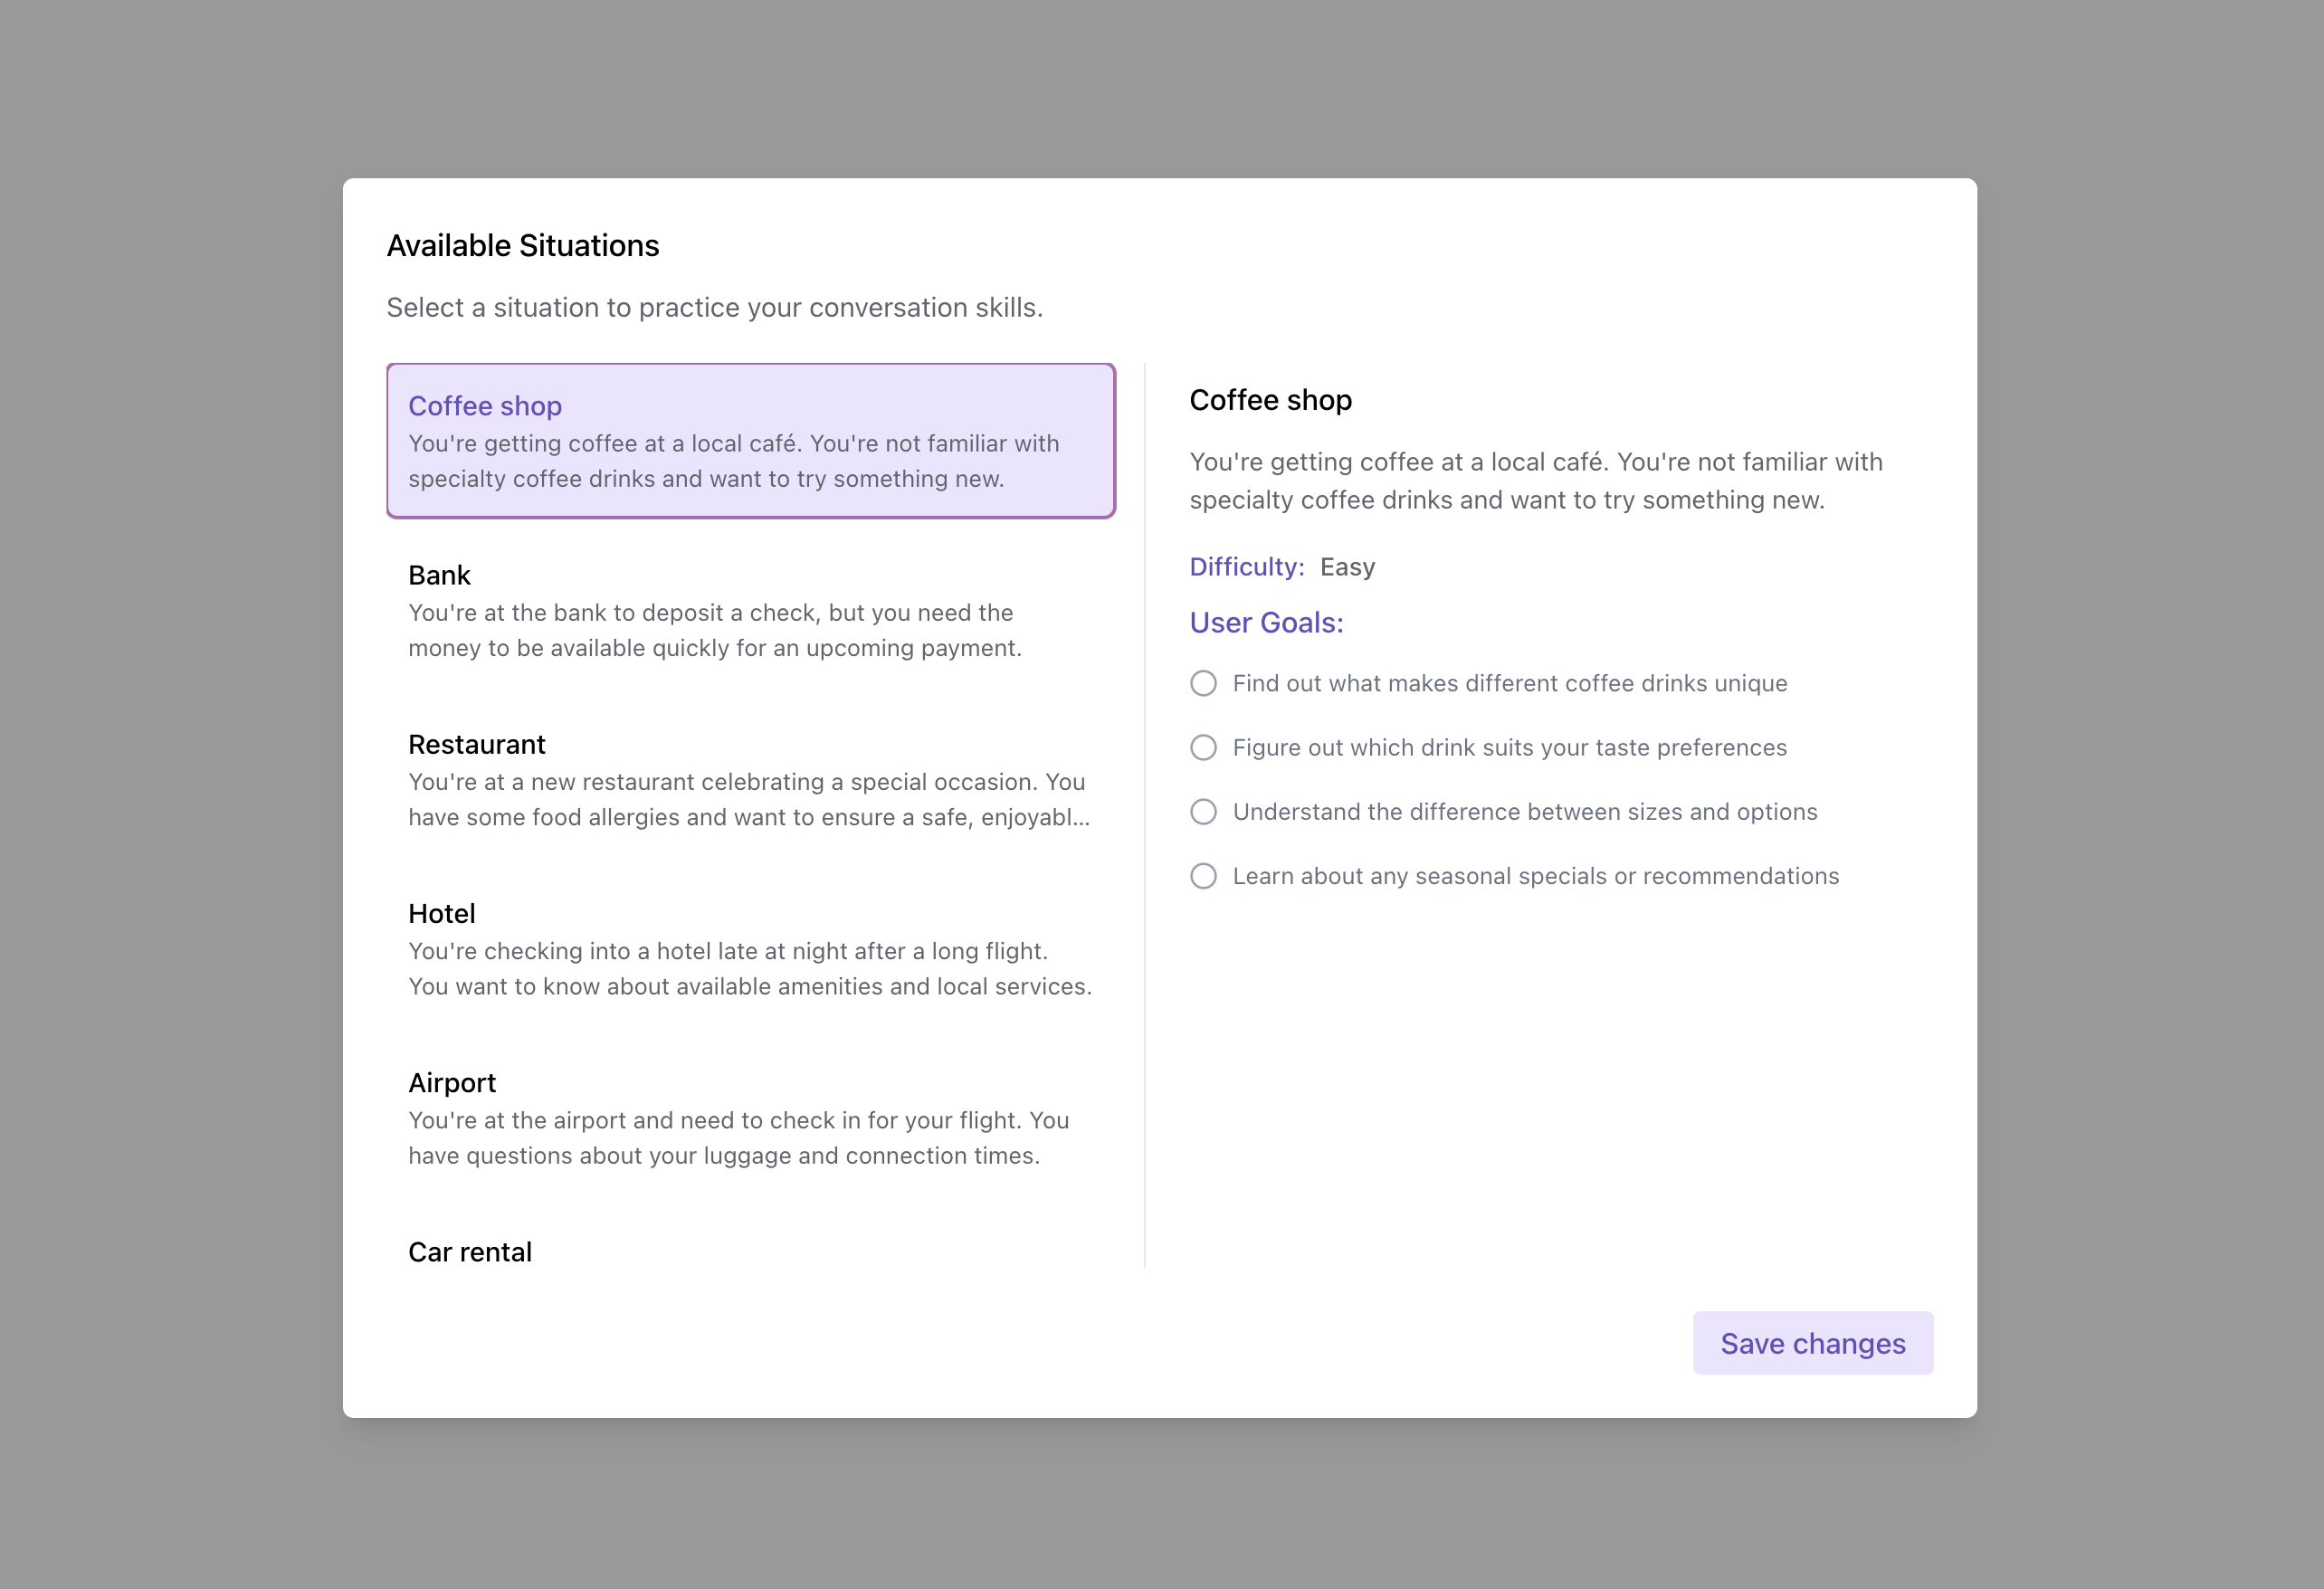
\includegraphics[width=0.8\textwidth]{figuras/screenshots/situation-picker.png}
    \caption{Interface for selecting conversational contexts and objectives}
    \label{fig:situation-picker}
\end{figure}

Figure \ref{fig:situation-picker} shows the situation selection interface, a key component for contextualized practice. This interface allows users to choose specific scenarios for their conversational practice, offering:

\begin{itemize}
    \item \textbf{Predefined Contexts:}
    \begin{itemize}
        \item Everyday scenarios such as restaurants, shops, and offices
        \item Professional situations for interviews and meetings
        \item Academic contexts for students
        \item Informal social situations
    \end{itemize}
    
    \item \textbf{Objectives System:}
    \begin{itemize}
        \item Clear list of communicative goals to achieve during the conversation
        \item Progress indicators for each specific objective
        \item Real-time feedback on progress toward goals
    \end{itemize}
    
    \item \textbf{Personalization:}
    \begin{itemize}
        \item Automatic adaptation of difficulty level according to the user's profile
        \item Recommendations based on practice history and areas for improvement
        \item Options to personalize specific objectives according to needs
    \end{itemize}
\end{itemize}

\subsection{Analysis Panel}
\label{panel-analisis}

\begin{figure}[H]
    \centering
    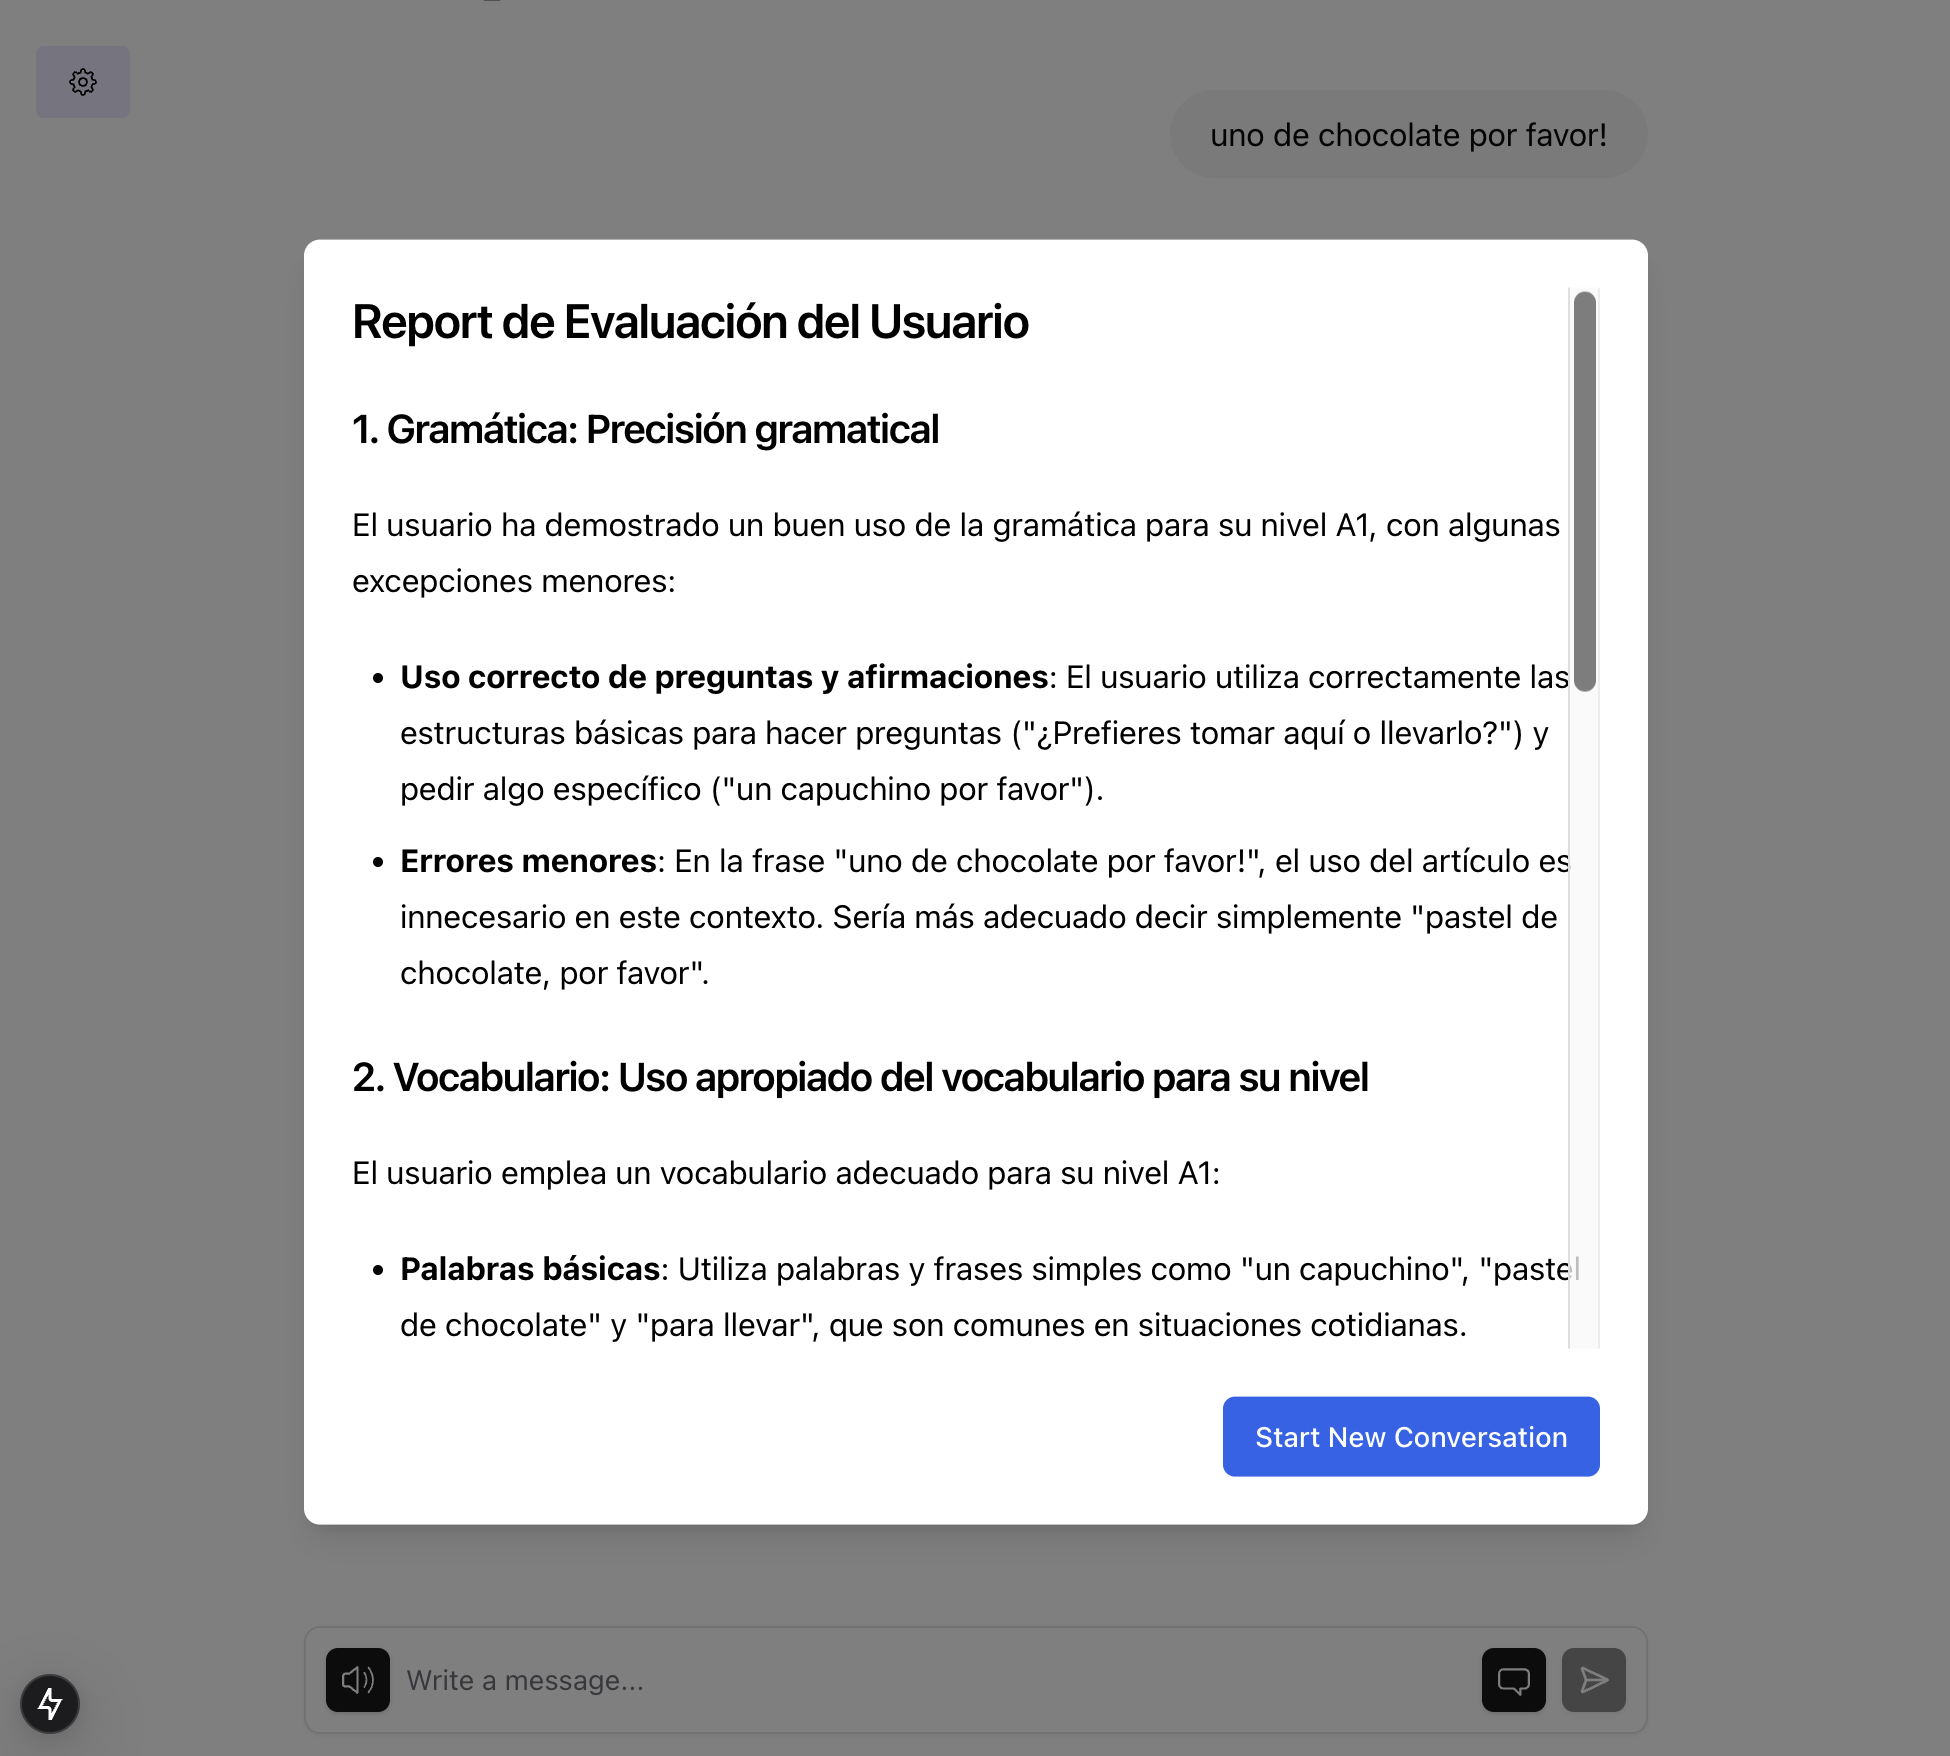
\includegraphics[width=0.8\textwidth]{figuras/screenshots/report.png}
    \caption{Analysis panel showing learning metrics}
    \label{fig:analytics-panel}
\end{figure}

Figure \ref{fig:analytics-panel} shows the results panel, designed to provide immediate feedback on conversation performance. This panel includes:

\begin{itemize}
    \item \textbf{Objectives achieved:} Record of goals reached during the conversation session.
    
    \item \textbf{Performance metrics:} Evaluation of the conversation in three key dimensions: grammar, vocabulary, and fluency, allowing the user to identify their strengths and areas for improvement.
    
    \item \textbf{Personalized report:} Detailed analysis of performance with specific observations on highlighted aspects and recommendations for improvement.
    
    \item \textbf{Continuity options:} The user can save their progress and later access the history page where they can visualize their evolution over time.
\end{itemize}

\subsection{Learning Progress Visualization}
\label{visualizacion-progreso}

\begin{figure}[H]
    \centering
    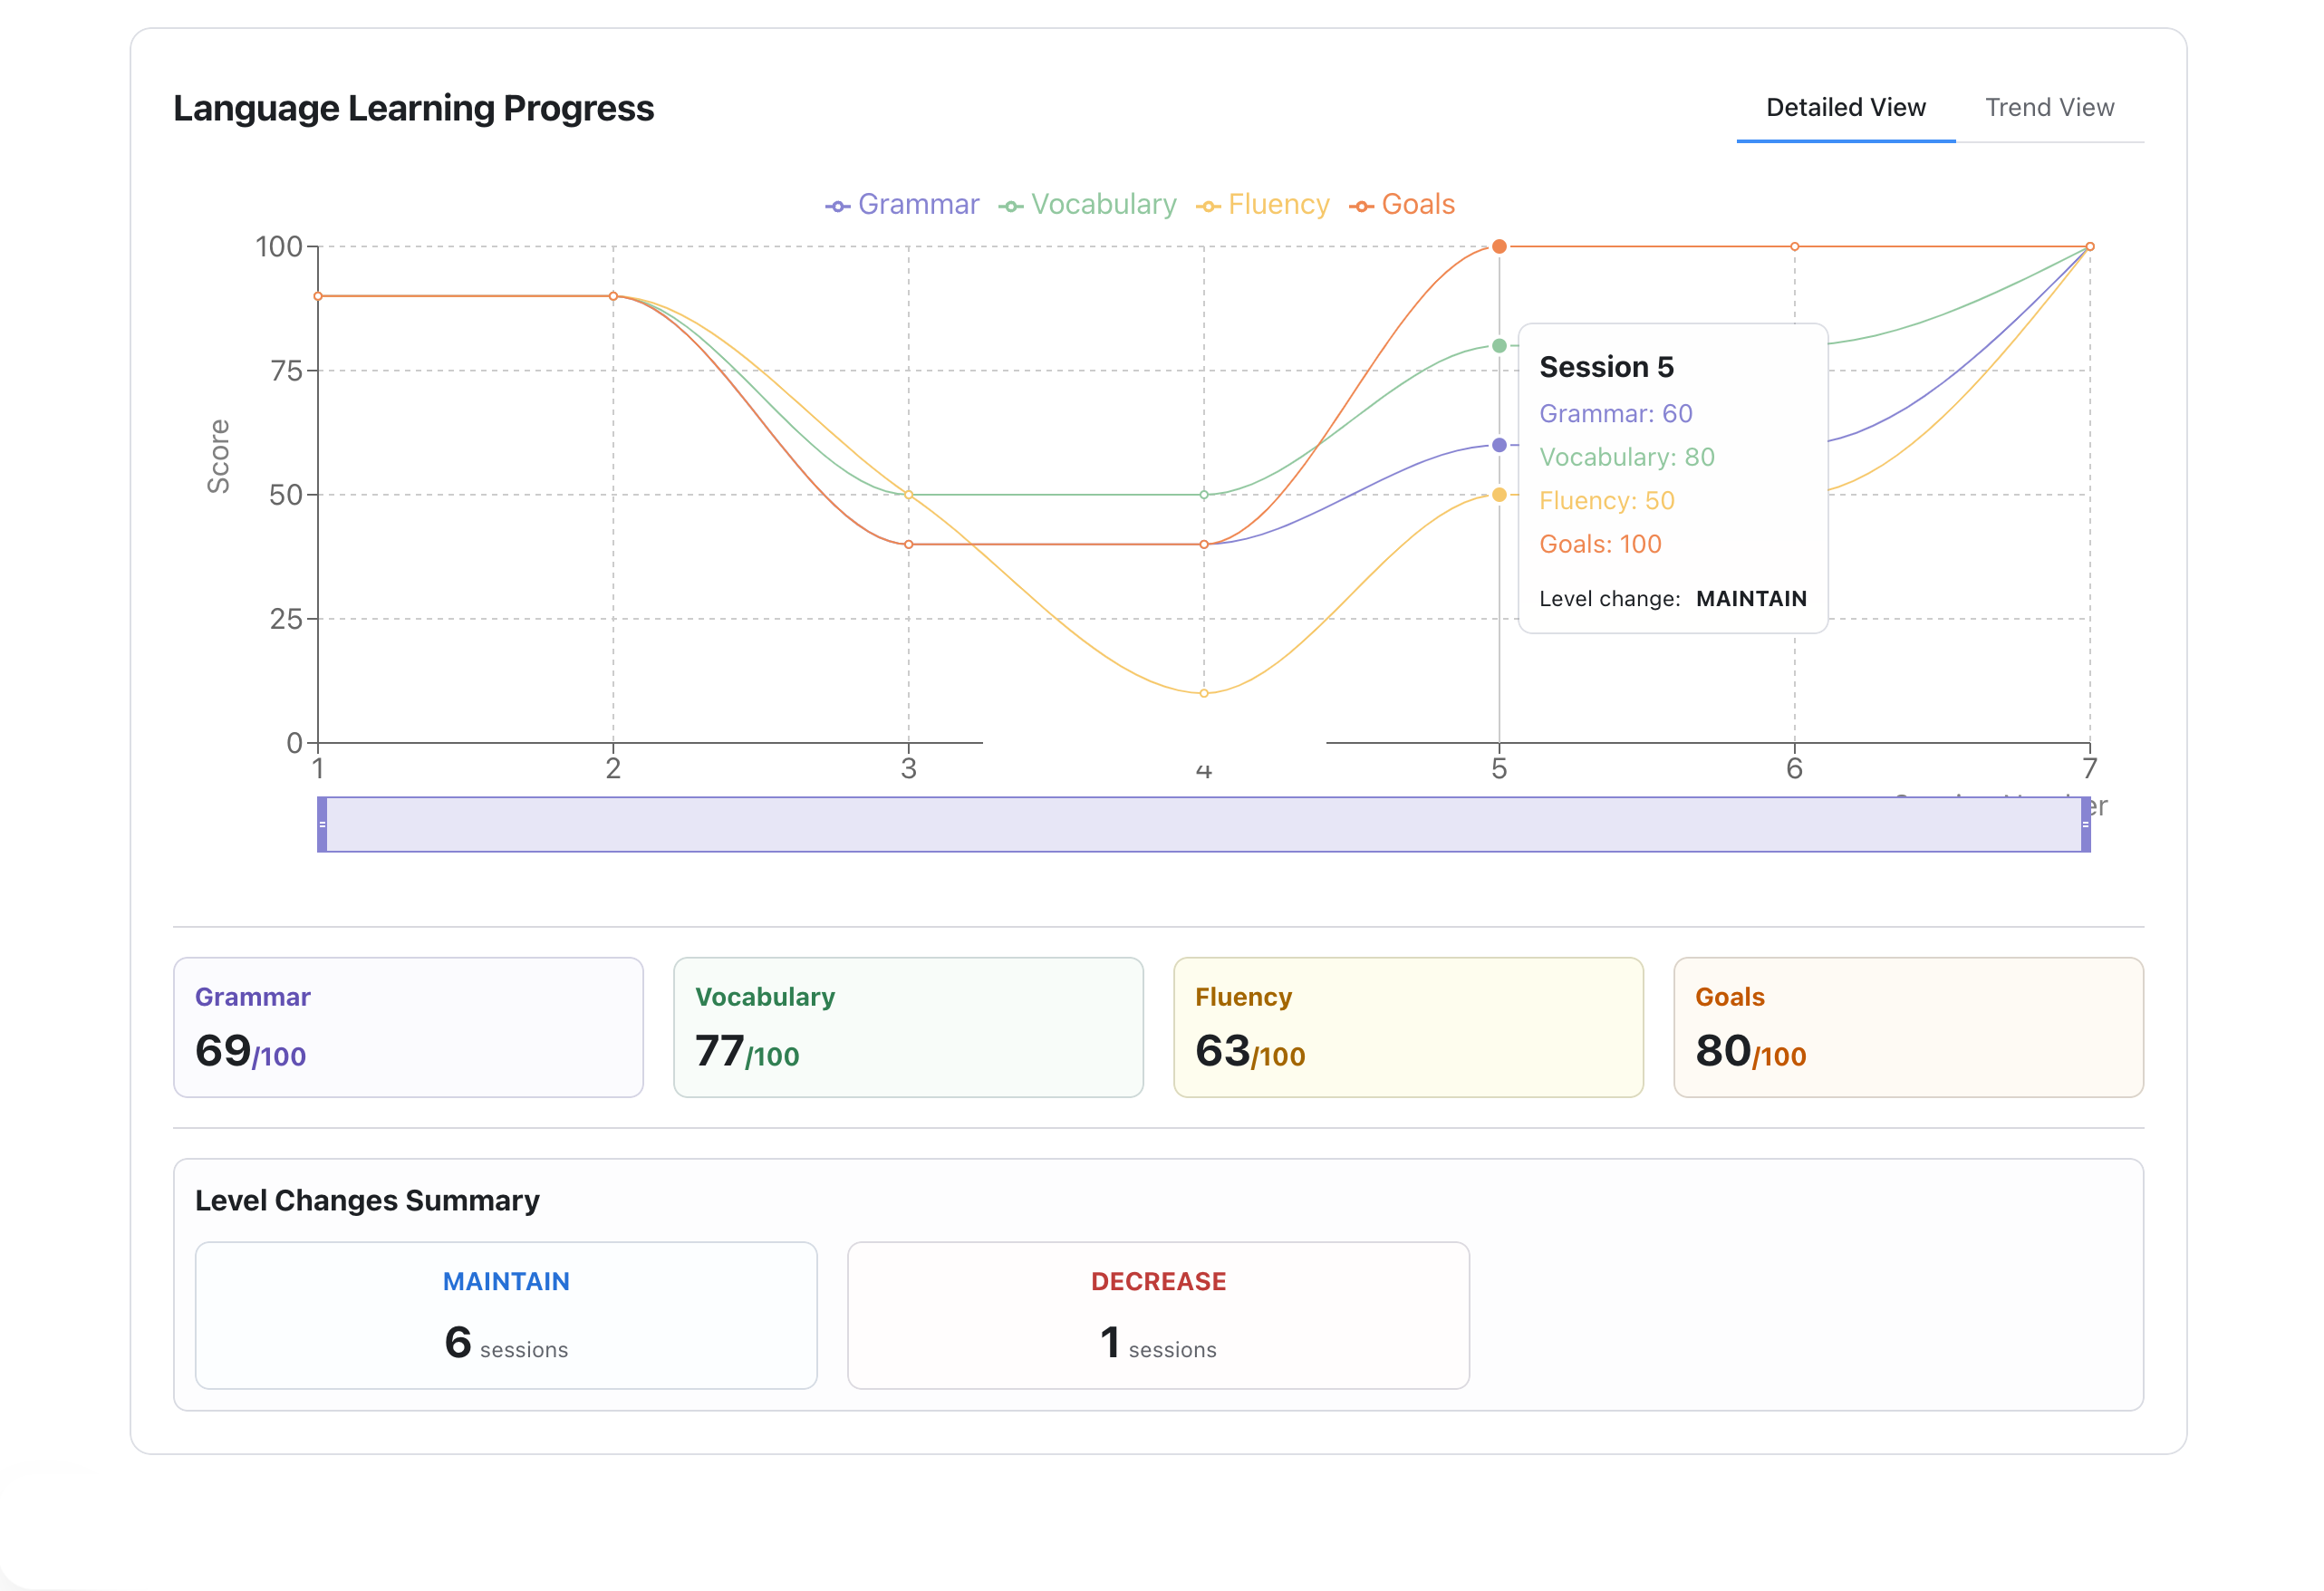
\includegraphics[width=0.8\textwidth]{figuras/screenshots/learning-history.png}
    \caption{Learning progress visualization interface with detailed metrics}
    \label{fig:learning-history}
\end{figure}

Figure \ref{fig:learning-history} shows the learning progress visualization interface, an essential component for tracking user performance. This tool provides a comprehensive graphical representation of linguistic development through various integrated functionalities.

\begin{itemize}
    \item \textbf{Flexible Temporal Analysis:} Combines a detailed view of individual sessions and a perspective of grouped trends, allowing the user to alternate between both modalities to identify both general patterns and specific details of their learning. The system incorporates interactive controls that facilitate chronological exploration of the data.
    
    \item \textbf{Comprehensive Evaluation of Linguistic Competencies:} Monitors four fundamental dimensions of learning: grammar, vocabulary, fluency, and fulfillment of communicative objectives. Each metric is presented visually using a consistent color code that facilitates comparison between skills and identification of strengths and areas for improvement.
    
    \item \textbf{Level Progression Analysis:} Offers a visual summary of the learning trajectory, categorizing sessions according to their results (level increase, maintenance, or decrease). This component provides statistical context on overall progress, allowing correlation of practice strategies with concrete results.
    
    \item \textbf{Adaptive and Accessible Design:} Implemented with Radix UI and responsive techniques to ensure an optimal experience on any device. The interface maintains the visual integrity of the data regardless of screen size, prioritizing accessibility through adequate contrast and well-defined interactive elements.
\end{itemize}

This progress visualization constitutes a fundamental tool for the student's metacognitive reflection, allowing them to identify patterns in their learning and make informed decisions about their future linguistic practices.

\section{Project Repositories}
\label{sec:repositorios-proyecto}

The system has been developed following a modern client-server architecture, with clear separation between presentation and business logic. All source code is publicly available on GitHub under the MIT license, promoting transparency, reproducibility, and community collaboration.

\subsection{Repository Structure}
\label{subsec:estructura-repositorios}

\begin{itemize}
    \item \textbf{Frontend - Client:}
    \begin{itemize}
        \item Repository: \url{https://github.com/EmaSuriano/language-learning-client}
        \item Technologies: Next.js 14, TypeScript, Tailwind CSS
        \item Main components:
              \begin{itemize}
                  \item Chat interface based on \gls{assistant-ui} with optimizations for learning
                  \item Situation and objectives selector with adaptive recommendations
                  \item State management with Zustand for efficient context handling
                  \item Internationalization system with i18n (support for 8 languages)
                  \item Optimized integration with audio API for voice processing
              \end{itemize}
    \end{itemize}

    \item \textbf{Backend - Server:}
    \begin{itemize}
        \item Repository: \url{https://github.com/EmaSuriano/language-learning-server}
        \item Technologies: FastAPI, Python 3.10, LangChain, Stable-Baselines3
        \item Main components:
              \begin{itemize}
                  \item \gls{rag} system for contextual retrieval of educational resources
                  \item Integration with \gls{llm} (Phi-4) for natural dialogue generation
                  \item \gls{api-rest} with OpenAPI documentation for client-server communication
                  \item Optimized implementation of Faster-Whisper and Kokoro-TTS
                  \item \gls{multi-agent} system based on LangChain for agent orchestration
                  \item \gls{ppo} model implemented with Stable-Baselines3 for level adaptation
              \end{itemize}
    \end{itemize}
\end{itemize}

\subsection{Documentation}
\label{subsec:documentacion-repositorios}

Both repositories include comprehensive documentation to facilitate understanding, use, and extension of the system:

\begin{itemize}
    \item \textbf{General Documentation:}
    \begin{itemize}
        \item Main README with project overview
        \item Detailed installation guides for development and production environments
        \item Architecture diagrams and data flow
        \item Contribution guides for external collaborators
    \end{itemize}
    
    \item \textbf{Technical Documentation:}
    \begin{itemize}
        \item Complete API specification through OpenAPI/Swagger
        \item Documentation of components and their responsibilities
        \item Required environment variables with examples and recommended configurations
        \item Guides for solving common problems
    \end{itemize}
    
    \item \textbf{Examples and Tutorials:}
    \begin{itemize}
        \item Usage examples for each main component
        \item Step-by-step tutorials for custom implementations
        \item Guides for extending existing functionalities
        \item Examples of integration with external systems
    \end{itemize}
\end{itemize}

This comprehensive documentation facilitates not only the reproducibility of the presented results but also the adaptation and extension of the system for different educational and linguistic contexts.

\section{Current Limitations and Future Work}
\label{sec:limitaciones-trabajo-futuro}

Despite the promising results obtained, it is important to recognize the current limitations of the system and define lines of future work to address them.

\subsection{Identified Limitations}
\label{subsec:limitaciones-identificadas}

\begin{itemize}
    \item \textbf{Technical Limitations:}
    \begin{itemize}
        \item Insufficient accuracy of the \gls{stt} system for strong non-native accents
        \item Relatively high initial system load time (5-8 seconds)
        \item Dependency on internet connection for advanced functionalities
        \item Significant computational resource consumption for low-end devices
    \end{itemize}

    \item \textbf{Pedagogical Limitations:}
    \begin{itemize}
        \item Limited coverage of domain-specific situations (technical, legal, medical)
        \item Evaluation system not yet validated with formal educational methodologies
        \item Insufficient adaptation to different learning styles
        \item Absence of mechanisms for collaborative learning among students
    \end{itemize}

    \item \textbf{Validation Limitations:}
    \begin{itemize}
        \item Reduced sample in preliminary tests (n=10)
        \item Relatively short evaluation period (2 weeks)
        \item Absence of control group for comparison with traditional methods
        \item Lack of longitudinal evaluation of the impact on learning
    \end{itemize}
\end{itemize}


\subsection{Future Work}

Based on the identified limitations and preliminary results, the following lines of future work are proposed:

\begin{itemize}
    \item \textbf{Comprehensive Evaluation:}
    \begin{itemize}
        \item Study design with expanded sample (n>100) and geographic diversification
        \item Implementation of longitudinal evaluation (3-6 months) to measure real impact
        \item Development of comparative methodology with control group using traditional methods
        \item Validation with language teaching professionals and pedagogy experts
    \end{itemize}

    \item \textbf{Technical Improvements:}
    \begin{itemize}
        \item Refinement of the \gls{ppo} model through fine-tuning with real user data
        \item Specific adaptation of the \gls{stt} system to improve accuracy with non-native accents
        \item Optimization of the \gls{rag} knowledge base with thematic expansion and automatic updating
        \item Implementation of offline modes for basic functionalities without connection
    \end{itemize}

    \item \textbf{Functionality Expansion:}
    \begin{itemize}
        \item Development of specific modules for specialized domains (business, tourism, academia)
        \item Implementation of social component for collaborative practice among students
        \item Integration with authentic content (news, videos, podcasts) for contextual immersion
        \item Development of adaptive gamification system to increase motivation and retention
    \end{itemize}
\end{itemize}

These lines of future work represent a structured plan to address current limitations and expand the capabilities of the system, with the aim of maximizing its educational impact and improving the learning experience for a wider range of users.

The results presented in this chapter, although preliminary, provide initial evidence on the viability and potential of the proposed approach. In the next chapter, the general conclusions of the work will be discussed, analyzing the contributions made, the lessons learned during development, and the broader implications of these advances for the future of technology-assisted language learning.